\documentclass[11pt]{article}
\usepackage{graphicx}
\usepackage{booktabs}
\usepackage{latexsym}
\usepackage{amsfonts}
\usepackage{amssymb}
\usepackage{amsmath}
\usepackage{amsthm}
\usepackage{verbatim}
\usepackage{setspace}
\usepackage{lscape}
\usepackage{multirow}
\usepackage{rotating}
\usepackage{array}
\usepackage{tabularx}
\usepackage{supertabular}
\usepackage[round]{natbib}
\usepackage[pdftex,pdftitle={Capital Structure Swaps},pdfstartview=FitH]{hyperref}
\usepackage{longtable}
\usepackage{fullpage}
\usepackage[colorinlistoftodos]{todonotes}
\newtheorem{hypothesis}{Hypothesis}
\newtheorem{lemma}{Lemma}
\newtheorem{proposition}{Proposition}
%\title{Capital Structure Swaps, Stochastic Liabilities, and Shareholder Wealth: The Case of Insurance}

\title{\textbf{Insurance Company Capital Structure Swaps \vspace{-2ex}\\and Shareholder Wealth}}

\author{James I. Hilliard\footnote{Contact Author, Assistant Professor of Finance, W.A. Franke College of Business, Northern Arizona University, Flagstaff, AZ 86011.  e-mail: james.hilliard@nau.edu, phone: (928) 523-7901. Dr. Hilliard gratefully recognizes support from the Spencer Educational Foundation and the Terry College of Business Terry-Sanford grant (University of Georgia).  Neither Spencer nor Terry-Sanford had any role in designing or conducting this research.}, Linda Schmid Klein\footnote{Professor of Finance Emeritus, University of Connecticut}, James R. Garven\footnote{The Frank S. Groner Memorial Chair of Finance and Professor of Finance \& Insurance, Baylor University}}
%\date{December 15, 2015}

\citestyle{jri}
\doublespacing
\begin{document}
\maketitle%\todo{consider new title when submitting to a journal}

\begin{abstract}
%\todo{rewrite abstract; make it more exciting}
In the face of asymmetric information and comparative advantage, there may be opportunities to enrich long-term shareholders at the expense of other stakeholders. While these opportunities will typically fade over repeated opportunities, the long-term nature of insurance claims may provide opportunities for market timing.  One way insurance managers can enrich long-term shareholders is by issuing equity to take advantage of favorable reinsurance market conditions. This is analogous to a traditional capital structure exchange (in which managers issue equity and use the proceeds to retire debt), except that the insurer's obligations are stochastic. Our model suggests that under certain conditions (especially when reinsurance appears ``cheap''), managers can enrich long-term shareholders by issuing more equity and using the proceeds to purchase reinsurance.

\end{abstract}

%\thanks{Under review at \textit{Geneva Risk and Insurance Review}.}
%\newpage


\section{Introduction}\label{sec:intro}

%\todo{don't start out with evidence. do a better job of discussing why a swap could add value.}
%\todo{Is swap the right word?}% 
Stock insurers face a unique capital market. The large bulk of an insurer's liabilities are policyholder claims on the firm's assets that are not fixed like straight debt. The policyholder can only make a claim when they experience a loss, and such losses are never certain. At the same time, regulators and ratings agencies monitor insurers to ensure that the firm will remain solvent even in the face of very large policyholder losses, increasing the probability that policyholder claims will be honored when they do arise.  One method available to insurers to satisfy regulators and others is reinsurance, in which the insurer will transfer a portion of their liabilities to a reinsurer, along with cash, and thereby fix their obligations to policyholders. We call such a transaction a ``capital structure swap.'' A similar, but opposite transaction could also be considered: a firm can issue new policies (subject to regulator approval) when insurance policies can command a premium (known as a ``hard market'') and use the proceeds to retire equity.

Furthermore, capital structure can be adjusted by changing the size of the asset base using dividend and cash management policies. Prior capital structure literature for insurers has not explored the impact of these capital sources on the capital structure decisions. In particular, this study explores the impact of information asymmetry and comparative advantage on the potential for capital structure arbitrage.

The seminal literature on capital structure \citep{modigliani1958a,modigliani1963a} suggests that in absence of frictions, capital structure does not affect firm value, and further that the tax-deductibility of interest payments causes debt to have a positive impact on post-tax earnings. However, work extending the theory to capital structure swaps in the presence of information asymmetry and other frictions is limited. Reinsurance purchase may have the effect of a capital structure swap that does not require any immediate public disclosure (i.e. using excess cash to purchase value-adding reinsurance rather than paying a dividend\footnote{Using slack cash to purchase reinsurance deploys retained earnings to retire liabilities (loss reserves).  Since this is an equity-for-liabilities trade, it has the same effect as a capital structure swap that issues equity to accomplish the same purpose. Following pecking order theory, using slack cash would be preferred since some transaction costs could be avoided.}) or requires disclosure of only one side of the swap (i.e. issuing stock and using the proceeds to purchase value-adding reinsurance.)

Moreover, there is conflicting evidence regarding the valuation effects of seasoned equity offerings in the insurance industry.  \citet{akhigbe1997a} found that the average two-day stock market valuation effects of insurer equity offerings between 1977 and 1992 are -0.32\%, and not significant at any standard level of significance.  Further, they find that these returns are significantly less negative than those of industrial comparison firms in a matched sample. In contrast, \citet{polonchek1995a} found that the average two-day stock market valuation effect of insurer equity offerings was -3.09\% and underperformed issuance effects of both banks and non-financial companies during the same time frame. \citet{polonchek1995a} use a sample of securities issues from 1975 to 1993 and attribute their result to the information asymmetry prevalent in the insurance industry, relative to that of commercial banks.  Since both studies employ a one-factor market model, with returns compared to a broad market portfolio, is it not clear why these finding diverge.  However, it is clear that \citet{akhigbe1997a} compare insurer returns with a matched set of industrial firms while \citet{polonchek1995a} compare them with the issuance-induced returns of all commercial banks during the same period. The predictions from this study suggest the use of proceeds from equity issues may explain some of this divergence.

In this article, we examine the impact of capital structure decisions of insurance companies on shareholder wealth under various conditions. We develop a model by which management can analyze changes in shareholder value resulting from issuing new policies or reinsuring existing policies. Consistent with prior capital structure work, we show that if management's estimates of asset values or loss reserve liabilities (including probability distribution) deviate from market estimates, they may be able to enhance the wealth of controlling shareholders by retiring or issuing equity. Second, we show that the correlation between the firm's asset returns and liability exposures will contribute to the relative impact of such a swap. 

The article proceeds as follows: section \ref{sec:motivation} discusses the opportunities for insurers to engage in capital structure swaps and highlights some of the market frictions that allow them to add shareholder value.  Section \ref{sec:lit} reviews prior capital structure swap literature. Section \ref{sec:model} develops the theoretical structure of the model, while section \ref{sec:results} presents numerical examples of several swaps, illustrating their results. Concluding remarks are offered in section \ref{sec:conclusion}.

\section{Motivation}\label{sec:motivation}

\citet{obrien2007a} show that, under certain conditions, issuing equity can enhance shareholder value. This finding deviates from much past literature on equity issues, most notably work by \citet{loughran1995a}, which shows that equity offerings provide poor returns relative to other investment opportunities. Results on capital structure swaps and exchange offers shown by \citet{masulis1980a} confirm this finding.  In this article, we exploit insurers' ability to change capital structure without signaling (by selling new policies to increase leverage or purchasing reinsurance to reduce leverage). The analysis is further motivated by the observation of \citet{babbel2005a}, who show that the market value of an insurer's assets is the sum of its franchise value and the market value of its tangible assets, while its market value of liabilities is the expected present value of the firm's liabilities. In our model, the firm's equity is an option to exchange its assets for its loss outcomes.  Thus, we extend the existing literature by examining the availability of reinsurance as a leverage-reducing tool for insurers in the context of insurance capital structure swaps.

The firm's franchise value in this model is the net present value of the fixtures that allow the firm to extract ``economic quasi-rents,'' including the firm's ability to generate business through its distribution network, charters, licenses, and reputation. Since a change in value resulting from a capital structure swap should not be affected by the presence or absence of the additional fixtures, we exclude them from our analysis without loss of generality. \citet{babbel2005a} model the value of the exchange option, but consider the present value of liabilities to be the present value of promised liability cash flows discounted at the risk-free rate. We further model the market value of liabilities as the difference between the market value of the firm and the value of the exchange option held by the firm's shareholders. Finally, the reinsurance market allows the firm to lay off risks in exchange for its payment equal to at least the market value of liabilities, thereby enabling leverage reduction without public announcement, possibly through a series of relatively small transactions.  By including the correlation between the insurer's assets and liabilities, we are able to examine situations in which the insurer can benefit from reinsurance simply due to the reinsurer's comparative advantage in bearing risk. We also examine the potential shareholder wealth effects from management exploiting information asymmetries between primary insurers and policyholders, as well as between primary insurers and reinsurers.

Prior research provides guidance in this study. \citet{fischer1978a} develops an extension to the Black-Scholes Option Pricing Model, in which the risk-free rate is replaced by the difference between the expected return on a hedge asset and the expected rate of increase of the exercise price of the option. However, difficulty finding an appropriate hedge asset for loss liabilities limits the usefulness of the Fischer model for this application. \citet{merton1973a} and \citet{margrabe1978a} suggest an extension of the Black-Scholes model that estimates the value of an option to exchange one asset for another, when the value of each asset is a random variable. Margrabe specifically suggests that this model is appropriate for valuing margin accounts, which accurately describes any firm with financial or operating leverage, including insurance companies. We will refer to this model as the ``Merton-Margrabe'' model.

Although \citet{weiss2004a} show that reinsurance, like insurance in general, is typically priced at levels above expected loss, \citet{mayers1990a} suggest that there may be times when reinsurance adds value for the ceding company. For example, insurers with concentrated ownership (Lloyd's in particular, as well as mutual insurers) and firms with less geographic concentration demand more reinsurance.  Thus, reinsurance purchase may result from comparative advantage in risk-bearing (the reinsurer has greater diversification opportunities) or efficiency in providing real services (economies of scale allow the reinsurer to provide underwriting and claims services at a lower price).  In particular, if the ceded losses have a low correlation with the reinsurer's loss pool, reinsuring these losses may reduce the volatility of the reinsurance firm, allowing the reinsurer to assume these risks at a lower premium than charged to the primary policyholder. This may be especially true for excess reinsurance, in which the cedant typically transfers only the tails of the claim to the reinsurer. Alternatively, the cedant may benefit from information asymmetry, if the ceding managers know the underwriting experience for the losses while the reinsurer does not. In such cases, the cedants may have a different estimate of either the ceded pool's expected loss, or a different estimate of the pool's volatility, or both.\footnote{Theoretically, such opportunities would be easier to exploit in one-shot games, since reinsurers would learn that they had made a bad bet and subsequently close the opportunity.  However, an insurer can get ``lucky'' for a limited number of consecutive periods, perpetuating the reinsurers' belief in the managers' estimates.} Any of these cases may create capital structure arbitrage opportunities similar to those suggested by \citet{obrien2007a}. Furthermore, unlike the signaling equilibrium problems in executing otherwise optimal publicly-traded security transactions, reinsurance purchases are not announced immediately but are revealed ex post in accounting and statutory reports. The absence of signaling effects relative to other capital structure transactions could intensify the incentives to purchase reinsurance.

\section{Literature Review}\label{sec:lit}

The seminal work of \citet{modigliani1958a} and \citet{modigliani1963a}, demonstrate that in a frictionless environment, firm performance is invariant to capital structure.  In addition, the cost of equity capital is a linear increasing function of the debt/equity ratio.  Thus, in equilibrium, capital structure swaps should not affect shareholder wealth. Specifically, according to \citet{miller1988a}, ``the sum of the values of all the claims is independent of the number and the shapes of the separate partitions.''

In later reviews of their work, \citet{miller1988a} and \citet{modigliani1988a} examine the potential of information content in dividend announcements and by extension, capital structure swaps.   As Miller suggests in his review paper, ``management-initiated actions on dividends or other financial transactions might then serve, by implication, to convey to the outside market information not yet incorporated in the price of the firm's securities.'' Indeed, the work of Modigliani and Miller shows that in the presence of both corporate and personal taxes, firms can theoretically carry extremely high leverage ratios in order to maximize shareholder wealth.  While banks and insurers are generally highly leveraged, the ability for such firms to keep leverage unsustainably high is mitigated by regulatory pressure.

\citet{rendleman1980a} and \citet{myers1984a} show how managers can exploit information asymmetry to transfer wealth from debtholders to shareholders in project selection and when debt is risky. In these cases, managers may have opportunities to use their information advantage to enrich shareholders, by using internal cash to finance transactions that investors may be unwilling to support in an equity issue.   \citet{staking1995a} and \citet{staking1997a} expand this discussion to the insurance industry and demonstrate that insurance managers can engage in another form of capital structure arbitrage be exploiting asset and liability duration mismatches within their portfolios.  

\citet{garven1987a} applies the earlier work on capital structure to the insurance industry.  He suggests that reinsurance is one way to adjust the insurance firm's capital structure, and consistent with \citet{modigliani1958a}, shows that in the absence of frictions, reinsurance is irrelevant when there are no frictions.  He models the impact of default risk and taxes on reinsurance purchase.  Consistent with \citet{modigliani1963a}, Garven finds that ceding insurers will purchase reinsurance to the extent that they can take advantage of tax shields.  Later work by \citet{garven2003a} finds empirical support for most of Garven's theoretical predictions. This observation is further motivated by \citet{doherty1981a}, who show a similarity between insurance policyholders and non-insurance risky corporate debt lenders. If policyholders are willing to pay a higher price for insurance when the probability of insurer ruin is lower, then insurers have an incentive to buy reinsurance.  Similarly, \citet{scordis2006a} demonstrate a number of operational (i.e. non-tax) benefits of reinsurance purchases, such as reducing information asymmetry, default probability or managers' rent-seeking behavior.  Also, \citet{mayers1990a} show that firms may purchase reinsurance when it creates tax advantages or reduces the cost of real services.  However, limited research exists examining the optimal capital structure changes for insurance companies when management has information that investors and reinsurers do not have.  In this paper, we extend the work of \citet{myers1984a} and \citet{rendleman1980a} to the specific project of reinsurance purchase by insurance companies.

\section{Theoretical Development}\label{sec:model}

Consider an insurance company where the assets are risk-free marketable securities and the liabilities are loss reserves. Management's objective is to maximize the wealth of controlling shareholders and they will undertake a capital structure adjustment when market conditions are favorable to achieve this end.  The model, as shown in figure \ref{fig:timeline} has three time points, $t=0$, referring to the time prior to the capital swap when market values of equity and liabilities are observed, $t=1$, referring to the time of the capital swap and $t=2$, referring to the future point at which the actual losses are known and paid. Any assets remaining at $t=2$ are distributed to the shareholders and the firm ceases to exist.\footnote{The timing and cash flows are similar in spirit to the models in \citet{palmon2007a} and \citet{brunner2006a}.}

The firm's controlling shareholders are those who own shares at $t=0$ and hold them to $t=2$. Other shareholders may exist at $t=0$ and $t=2$, but management is not constrained to consider their wealth objectives in the capital swap (this suggests that the controlling shareholders may benefit at the expense of intermediate or future noise traders). Nor is management constrained to consider the wealth objectives of policyholders, except to honor their contractual obligations and maintain regulatory compliance.\footnote{It is important to note the limits of such a model.  In general, as this study analyzes optimal managerial behavior in discrete time period, and further assumes dissolution of the firm at the end of that period, the results do not easily generalize to a long-lived firm with multiple financing opportunities and infinite life.  If this model were extended to multiple periods, the reinsurer(s) would eventually learn the insurer was sending bad risks and adjust prices accordingly. However, even with this limitation, the study is a useful exercise, as it demonstrates how a firm might act in cases of financial distress or when management has private information relative to the distribution of their firm's loss distribution. Furthermore, since the outcome is by definition random, the ``lucky'' insurer may be able to replicate such a strategy a few times before being discovered. The rational reinsurance decision in a repeated game is a subject for future research.}

\begin{figure}[ht]\caption{Capital Restructuring Model Timeline\label{fig:timeline}} % title of the Figure
\begin{small}Model timeline in which $E_M$ is the market valuation of the firm, given publicly available information.  $E_I$ is management's estimate of the firm's equity value, given their private information.\end{small}
\setlength{\unitlength}{0.14in} % selecting unit length

\begin{center}\leavevmode % used for centering Figure
\begin{picture}(30,6.5) % picture environment with the size (dimensions)
% 40 length units wide, and 8 units high.
\put(1,4){\framebox(6,3){$t=0$}}
\put(11,4){\framebox(6,3){$t=1$}}
\put(21,4){\framebox(6,3){$t=2$}}
\put(7,5.5){\vector(1,0){4}}
\put(17,5.5){\vector(1,0){4}}
\put(1,-0.05){\makebox(6,3){Observe Expected Losses}}
\put(1,-1.5){\makebox(6,3){$E_M \ne E_I$}}
\put(11,-0.15){\makebox(6,3){Capital }} 
\put(11,-1.5){\makebox(6,3){Structure Swap}}
\put(21,-0.15){\makebox(6,3){Pay Claims}}
\put(21,-1.5){\makebox(6,3){$E_M = E_I$}}
\end{picture}
\end{center}

\label{fig:model} % label to refer figure in text
\end{figure}

In our model, at $t=0$, management has his own estimated probability distribution of claims that he believes to be true, including the volatility of the loss reserves. Management also observes the price of reinsurance and the market price for new policies, reflecting the market estimate of the claim loss distribution.  Any discrepancy between management's estimate and the market's estimate of loss volatility is expressed as $\beta$ ($\beta>0$; if there is no discrepancy about volatility estimates, then $\beta=1$. If $\beta>1$, then the market estimate of volatility is higher than management's estimate). Similarly, discrepancy between manager and market estimates of expected loss is expressed as $\gamma$ and discrepancy between manager and market estimates of asset/loss correlation is expressed as $\delta$. Based on observing such deviations, management determines whether an opportunity exists to increase the wealth of controlling shareholders by issuing or retiring equity and either purchasing reinsurance (i.e. laying off the risk at the cost of a certain payment and reducing liabilities) or issuing more policies (i.e. increasing liabilities). Management also observes market values for the company's equity and loss reserves (i.e. the cost of purchasing reinsurance on part or all of its book of business).  When management issues equity, they use the proceeds to reduce expected loss at a rate of $\alpha$ ($0<\alpha<=1$) by purchasing a pro-rata reinsurance policy, in which the reinsurer assumes a $1-\alpha$ proportion of the loss reserve in exchange for cash generated by the equity issue.  Conversely, when management retires equity, they market and sell new policies, increasing expected loss at a rate of $1+\alpha$ and using the proceeds to retire equity. At $t=1$, the capital restructuring occurs (losses increase or decrease by a factor of $\alpha$) and at $t=2$, all policies expire, claims are paid and any remaining loss reserves and other assets are distributed to the $t=2$ equity holders.

We begin with an assumption that the value of the firm's equity is the net value of its assets less the expected losses in its policy portfolio.  This value remains constant until the random outcome is known at $t=2$ and losses are paid out.  Therefore, a change in the value of liabilities (brought about by either issuing more policies or reinsuring some portion of the book) at $t=1$ will require an equal and opposite change in the value of the equity. We assume that management will not over-insure, that is, reduce expected losses below 0. Note that the difference between the management's estimate of equity value and the market estimate of equity value may reflect management's private information about the probability distribution of the loss pool and asset values or correlation between loss reserves and assets.\footnote{Following \citet{myers1984a}, we assume the existence of perfect capital markets that are efficient with respect to publicly available information; this implies that the current market value of the firm corresponds to the discounted value of its expected future cash flows, conditional upon whatever publicly available information the market happens to possess about the firm. Since private information held by corporate insiders is idiosyncratic (and therefore diversifiable), the existence of such information does not affect current market value.}  The insurer's volatility estimate reflects the total risk of the loss, subject to the diversification benefits of its own portfolio, while the market estimate of volatility reflects only market risk, as market prices should not reflect diversifiable risk. When these values differ, management may have an opportunity to engage in a capital swap that he believes will enrich the controlling shareholders.\footnote{Note that such an exchange does not necessarily represent an arbitrage opportunity, but an action based on different expectations regarding probability distributions.  Controlling shareholders may indeed lose money as a result of such an action, but management is acting based on their own beliefs and assumptions about the dynamics of the firm's loss portfolio.}

\begin{equation}\label{eqn:basevalue}
E_j=A_j-L_j
\end{equation}

In Equation \ref{eqn:basevalue}, $E$ is value of equity, $A$ is value of tangible assets and $L$ is the present value of expected claims. The subscript $j$ is either $M$ (market value) or $I$ (insider value).  If the assets of the firm are investments in the market portfolio, they can be readily valued without dispute and market values equal insider values.\footnote{If the insurer does not hold the market portfolio on the asset side, there may be additional opportunities for capital structure arbitrage that are not modeled here.} We are left with $E_j$ sensitive to only $L_j$. When the estimates of expected losses differ, management's estimate of firm equity value is defined by Equation \ref{eqn:intrinsicvalue}:

\begin{equation}\label{eqn:intrinsicvalue}
E_I=A-L_I
\end{equation}

And the market value is defined by Equation \ref{eqn:marketvalue}:

\begin{equation}\label{eqn:marketvalue}
E_M=A-L_M
\end{equation}

In a competitive market regulated both by state insurance departments and the Securities and Exchange Commission, some might argue that differences between the insider value and the market value of expected losses should rarely exist.  However, \citet{weiss2004a} suggest that probability updating for losses may drive such differences. The 2003 restatement of reserves for asbestos exposure exemplifies revaluation of loss reserves across the industry. As firms realized that their previous estimates of asbestos exposure were incorrect, they re-stated the true expected loss related to asbestos. Prior to the completion of these reserve analyses, the market estimated the value of the losses higher than the firm.  Differences between the insider's estimate of loss variability and the market estimation of variability may exist in other instances. For example, management observes the details of the policy and thus may have a better estimate of the insureds' loss distributions. At the same time, the market can only estimate the policy characteristics under limited access to the underwriting files, prior loss experience, regulatory filings and ratings agency estimates.

Indeed, even if both the firm and the market agree on underlying loss distribution, the correlation between assets and losses may drive differences in loss valuation. That is, a prospective policyholder may have potential losses that are highly correlated with their asset holdings.  They would value an insurance policy differently than an insurer with greater access to capital, and greater ability to diversify by retaining the loss exposure on its balance sheet.  For personal lines policyholders and closely-held commercial lines policyholders, the role of risk aversion will also factor into the reservation price for insurance.

\citet{doherty1986a}, \citet{babbel2005a} and \citet{obrien2004a} show that when asset returns are risk-free and loss distributions are uncertain, the value of the firm's equity is the value of an option to exchange the firm's assets for the policyholders' losses, with the strike price being the future value of the assets. The option can be valued using the standard Black-Scholes option pricing model.  

In cases where either the market's estimation of expected loss or asset return volatility differs from management's estimation (the insider value), management may consider making a capital structure swap to enhance the wealth of $t=0$ shareholders who will hold their shares until $t=2$.

\subsection{Valuation When Assets and Liabilities are Risky}

As shown by \citet{rubinstein1976a} and \citet{cox1979a}, 
option pricing principles
% the Black-Scholes option pricing model (and by extension, its derivative models such as the Merton-Margrabe model) 
can be used to value capital budgeting projects and securities with or without limited liability. If the insurer is investing its assets in at least some risky securities, the strike price for the exchange option is also a random variable and can be valued using ``preference-restricted''\footnote{\citet{Stapleton1984} show that it is not necessary to rely upon standard no-arbitrage justifications for applying models such as Merton-Magrabe to the analysis of this particular problem. Specifically, the functional form of the Merton-Margrabe model still obtains so long as assets and liabilities are jointly lognormally distributed, \textit{and} investors have constant relative risk aversion (CRRA) preferences, which is what we assume here.} version of the Merton-Margrabe model (cf. \citet{merton1973a} and \citet{margrabe1978a}). The Merton-Margrabe model shows that an option to exchange one risky asset for another can be valued according to the following formula:\footnote{\citet{fischer1978a} derives a model similar to \citet{merton1973a} and applies it to the valuation of indexed bonds.  Insurance loss reserves are essentially indexed bonds, with the final payoff being indexed to the cost of settling any losses.} 

\begin{equation}\label{eqn:valuation}
E_j=A_j N\left(d_1 \right)-L_j N \left(d_2 \right)
\end{equation}

\noindent In equation (4), $E_j$ is value of equity, $A_j$ is current value of assets and $L_j$ is expected value of loss liabilities. The function $N \left(\bullet \right)$ is a draw from the standard normal distribution function.
\begin{displaymath}
d_{1j}=\frac{ln \left(\frac{A_j}{L_j} \right)+0.5 V_j^2 t}{V_j \sqrt{t}}, 
d_{2j}=d_{1j}-V_j \sqrt{t}
\end{displaymath}
\begin{displaymath}
V_j^2=\sigma_{jA}^2+\sigma_{jL}^2-2 \rho_{jAL}\sigma_{jA} \sigma_{jL}
\end{displaymath}
$j$ takes the value of $M$ for market value of equity and $I$ for insider value of equity, $\sigma_{jk}$ is the standard deviation of the variable $k$ (either $A$ for assets or $L$ for losses) under $j$, and $t$ is time to policy expiration. Thus, market estimates of pre-swap equity values would be:

\begin{displaymath}
d_{1M}=\frac{ln\left(\frac{A}{\gamma L}\right)+0.5V_M^2 t}{V_M\sqrt{t}}, d_{2M}=d_{1M}-V_M\sqrt{t}
\end{displaymath}
\begin{displaymath}
V_M^2=\sigma_A^2+\beta^2\sigma_L^2-2\delta\rho_{AL}\sigma_A\beta\sigma_L
\end{displaymath}
Note that $V_j^2$ is the instantaneous variance (estimated separately by management and investors) of the portfolio of long assets and short liabilities, and for simplicity, probability distributions for assets and liabilities are stable over time.\footnote{Some may suggest that these models require continuous trading and publicly tradable securities.  First, as already shown, \citet{rubinstein1976a} derives the option pricing model in a discrete time framework.  Second, while it may not seem obvious at first, loss reserves are increasingly tradable.  There has been a liquid reinsurance market in the developed world for decades, constantly swapping risks and trading risk for cash.  In addition, the past decade has seen the proliferation of loss securitization, in which losses are bundled and sold to investors in exchange for LIBOR plus risk premium coupons.  Thus, these constraints should not apply to use of an option pricing model in this context.}  

\subsection{The Swap}
When management chooses to undertake a capital structure swap, they will essentially increase or reduce the expected value of the loss reserves by some proportion $\alpha$.  When $0<\alpha<1$, management is purchasing reinsurance funded by an equity issue.  When $\alpha > 1$, management is issuing new policies and using the proceeds to retire equity.  Thus, managers believe that the post-swap value of the firm is adjusted by $\alpha$, investors will evaluate the change in value based on their estimates of $\beta$, $\gamma$ and $\delta$. In the context of equation \ref{eqn:valuation}, we propose lemma \ref{lemma:equitypartiala}.

\begin{lemma}\label{lemma:equitypartiala}
The post-swap value of equity is a decreasing function of $\alpha$.
\end{lemma}

\begin{proof}
The relationship between post-swap value of equity and $\alpha$ is determined by taking the partial derivative of equity:

\begin{eqnarray}
\frac{\partial E}{\partial \alpha}&=&A \frac{\partial N\left(d_1\right)}{\partial d_1}\frac{\partial d_1}{\partial \alpha}-\delta L \left[N\left(d_2\right)\right]-\alpha \delta L \frac{\partial N\left(d_2\right)}{\partial d_2}\frac{\partial d_2}{\partial \alpha}
\end{eqnarray}

Note that:
\begin{eqnarray}
\frac{\partial N\left(d_1\right)}{d_1}&=&n\left(d_1\right) \nonumber\\
\frac{\partial d_2}{\partial \alpha}&=&\frac{\partial d_1}{\partial \alpha} \nonumber\\
\frac{\partial d_1}{\partial \alpha}&=&-\frac{1}{\alpha V \sqrt{t}} \nonumber\\
d_1&=&\frac{\ln\frac{A}{\alpha \delta L}+0.5 V^2 t}{V\sqrt{t}} \nonumber \\
\mbox{therefore} &&\nonumber \\
d_1 V\sqrt{t}&=&\ln\frac{A}{\alpha \delta L}+0.5 V^2 t\nonumber\\
d_1 V\sqrt{t}-0.5 V^2 t&=&\ln\frac{A}{\alpha \delta L} \nonumber\\
A&=&\alpha \delta L e^{d_1 V\sqrt{t}-0.5 V^2 t }
\end{eqnarray}

Therefore, 
\begin{equation}
\frac{\partial E}{\partial \alpha}=A \frac{n\left(d_1\right)}{\alpha V \sqrt{t}}-\delta L\frac{n\left(d_1-V\sqrt{t}\right)}{V\sqrt{t}}-\alpha \delta L \left[N \left(d_2\right)\right]
\end{equation}
Substituting for $A$ and expanding the $n$ operator:
\begin{eqnarray}
\frac{\partial E}{\partial \alpha}&=&-\frac{\alpha \delta L}{\alpha V\sqrt{2t \pi}} e^{d_1 V\sqrt{t}-0.5 V^2 t} e^{-0.5 d_1^2} -\frac{\delta L}{V\sqrt{2t \pi}}e^{-0.5\left(d_1-V\sqrt{t}\right)^2}-\alpha \delta L \left[N \left(d_2\right)\right] \nonumber\\
&=&-\frac{\delta L}{V\sqrt{2t \pi}}\left(e^{-0.5\left(d_1-V\sqrt{t}\right)^2}-e^{-0.5\left(d_1-V\sqrt{t}\right)^2}\right)-\alpha \delta L \left[N\left(d_2\right)\right]\nonumber\\
&=&-\alpha \delta L \left[N\left(d_2\right)\right]
\end{eqnarray}

Thus, as long as liabilities are positive, equity value decreases in proportion to liabilities changed and any deviation between insider and market estimates of expected loss.

\end{proof}
Two examples follow in which expected management estimates of  volatility and expected loss (policy face value) differ from market estimates.

If management believes that reinsurance will add value for the firm, they may be able to enrich controlling shareholders by purchasing reinsurance with the proceeds of a new equity issue.  However, a firm can use excess cash to adjust to a desired capital structure without incurring flotation costs. Alternatively, management could enrich controlling shareholders by selling more policies, using the proceeds to reduce outstanding equity and thereby increase leverage if they believed that they could sell policies at a sufficient premium or retire equity at a sufficient discount.  Management need not retire equity to make such a swap worthwhile; they could instead use policy-generated cash to finance new projects or increase capital levels to satisfy regulators.

Efficient market theory, especially \citet{ross1977a}, suggests that  announcement of an equity issue or equity repurchase should signal management's private information to the market and prices should immediately adjust to reflect that new information.  However, empirical evidence (See, for example, \citet{lakonishok1990a,ikenberry1995a,loughran1995a,speiss1995a}, and other literature summarized by \citet{klein2002a}) suggest that market responses are not necessarily immediate.  With particular application to insurance companies, \citet{miller2005a} find that positive excess returns persist for several months following equity repurchase announcements. 

In order to test the impacts of capital structure shifts, we assume that management will undertake these transactions without signaling frictions (for example, purchasing reinsurance or issuing new policies) and that the market will become aware of the loss reserve outcome at $t=2$.\footnote{Becoming aware of the outcome does not indicate that either management or the market actually knew the \textit{a priori} loss distribution.}  Benefits accruing to controlling shareholders will decline in the presence of signaling frictions.\footnote{This model assumes no other frictions.  Any transaction costs associated with purchasing reinsurance (a premium loading by the reinsurer to cover administrative expenses and premium taxes) or selling policies (commissions paid to agents and brokers, as well as premium taxes), will further reduce any benefit to controlling shareholders, and may reverse the benefit if those costs are high enough.} At $t=1$, management is maximizing shareholder wealth given expectations of $t=2$ outcomes.  Since all outcomes will become known at $t=2$, the market value and the insider value will be  equal, $E_{M, t=2}=E_{I, t=2}$, so we will suppress the $j$ subscript for expected values at $t=2$.

The intuition for this analysis is clearest when we assume that the manager purchases reinsurance on a pro-rata basis.  That is, the manager will cede some portion of its loss reserve.  There is no disagreement on the proportion of the book being reinsured, so that a 20\% pro-rata policy reduces both insider estimate of loss by 20\% and the market estimate of loss by 20\%.  The proportion of the book being reinsured is indicated by $\alpha$, which is constant over all periods and agreed upon by all participants.

To motivate our signaling friction restrictions, consider a firm whose controlling shareholders have superior information, perhaps by virtue of board seats or managers with significant equity stakes\footnote{We recognize the contribution of Jos\`{e} Manuel Campo for this illustration.}.  The managers of such a firm, with compensation tied to changes in the final value of shares held by these controlling shareholders, may seek to expropriate wealth from less informed noise and liquidity traders. This can be done by issuing or retiring equity when they believe the market conditions are best suited to maximizing controlling shareholder wealth. Furthermore, insurance companies typically hold cash and marketable securities in sufficient quantity such that equity market transactions need not be contemporaneous with cash flow shocks within the firm.

The definition of terminal controlling shareholder wealth depends on the type of swap.  When the firm issues equity and uses the proceeds to buy reinsurance, the $t=2$ wealth of controlling shareholders ($W_{t=2}$) is the ratio of market value of equity at $t=0$ to market value of equity at $t=1$, multiplied by the value of the firm's equity at $t=2$.

\begin{equation}\label{eqn:issueequity}
W_{t=2}=\frac{E_{M,t=0}}{E_{M,t=1}}E_{t=2}
\end{equation}

Where $W_{t=2}$ is the shareholder wealth at $t=2$ and $E_{jt}$ is the $j$ value of equity at time $t$. Equation \ref{eqn:issueequity} represents the proportion of total equity market value before the swap (held by the controlling shareholders) to total equity market value after the swap (held by both controlling shareholders and noise traders). Thus the ratio reflects the smaller proportion of total equity market value held by the controlling shareholders after the swap has occurred.  This ratio is then multiplied by the total $t=2$ equity value to represent the terminal wealth of the controlling shareholders.  New shareholders have been added, and the controlling shareholders now hold a smaller portion of the total equity than they held before the swap occurred.  Management will engage in the swap only when the optimal $t=2$ wealth exceeds the $t=0$ wealth.

When the firm issues new policies and uses the proceeds to retire equity, the initial wealth of controlling shareholders is the ratio of market value of equity at $t=2$ to the market value of equity at $t=0$, multiplied by the $t=0$ insider value of the firm's equity:

\begin{equation}\label{eqn:retireequity}
W_{t=0}=\frac{E_{M,t=1}}{E_{M,t=0}}E_{I,t=0}
\end{equation}

Equation \ref{eqn:retireequity} represents the proportion of total equity market value after the swap to total equity market value held before the swap, and reflects the ratio of total equity held by the controlling shareholders.  This ratio is then multiplied by the total $t=0$ insider equity value to represent the wealth of the controlling shareholders prior to the swap.  The controlling shareholders hold a larger portion of the equity after the swap than they held before the swap occurred.  Again, management will engage in the swap only when the the $t=2$ wealth exceeds the $t=0$ wealth.

For firms issuing equity and using proceeds to purchase reinsurance, the change in controlling shareholder wealth as a function of expected losses is:

\begin{eqnarray}\label{eqn:maxissuefull}
\frac{\partial
\displaystyle\left[\frac{E_{M,t=0}}{E_{M,t=1}}E_{t=2}\right]}{\partial\alpha}&=&\left(\frac{E_{M,t=0}}{E_{M,t=1}}\right)\left(\frac{\partial E_{t=2}}{\partial \alpha}\right)-\left(\frac{E_{t=2}E_{M,t=0}}{E^2_{M,t=1}}\right)\left(\frac{\partial E_{M,t=1}}{\partial \alpha}\right) \nonumber \\
&=& \left(\frac{E_{M,t=0}}{E_{M,t=1}}\right) \left[\frac{\partial E_{t=2}}{\partial \alpha}-\left(\frac{E_{t=2}}{E_{M,t=1}}\right)\left(\frac{\partial E_{M,t=1}}{\partial \alpha}\right)\right]
\end{eqnarray}

The unsimplified version of equation \ref{eqn:maxissuefull} represents the intuition: The first term on the right-hand side represents the change in value of the controlling shareholders' equity value for each unit change in expected loss, while the second term represents the cost or benefit (dilution or accretion) resulting from the equity issue. If a value of $\alpha$ can be found that sets makes these two terms are equal, there is an optimal swap. The second version facilitates signing the derivative and predicting the change. The ratio outside the square brackets is strictly not negative since, as option values, neither the numerator nor denominator can be negative.  By lemma \ref{lemma:equitypartiala}, the first term inside the brackets is negative, and the second term is positive (since the partial derivative is negative).   The only thing management must determine, then, is under what circumstances the second term inside the brackets is larger in absolute value than the first.  

When retiring equity, we take the partial derivative of equation \ref{eqn:retireequity} with respect to $\alpha$, as follows:

\begin{eqnarray}\label{eqn:maxretirefull}
\frac{\partial
\displaystyle\left[\frac{E_{M,t=1}}{E_{M,t=0}}E_{I,t=0}\right]}{\partial\alpha}&=&\left( \frac{E_{M,t=1}}{E_{M,t=0}}\right)\left(\frac{\partial E_{I,t=0}}{\partial \alpha}\right)-\left(\frac{E_{I,t=0}E_{M,t=1}}{E^2_{M,t=0}}\right)\left(\frac{\partial E_{M,t=0}}{\partial \alpha}\right)\nonumber\\
&=&\left(\frac{E_{M,t=1}}{E_{M,t=0}}\right)\left[\frac{\partial E_{I,t=0}}{\partial \alpha}-\left(\frac{E_{I,t=0}}{E_{M,t=0}}\right)\left(\frac{\partial E_{M,t=0}}{\partial \alpha}\right)\right]
\end{eqnarray}

Again, the unsimplified version of equation \ref{eqn:maxretirefull} provides an intuitive explanation: the first term represents the change in the controlling shareholders' portion of the post-swap equity. The second term represents the increase in shareholder wealth that accumulates from the reduced number of shares outstanding.

Let us first consider, for example, the case in which management believes that the volatility of the loss pool is lower than market valuations suggest.  We will refer to this deviation as $\beta>1$, where $\beta=1$ indicates no disagreement.  Option valuation mechanics suggest that option value increases in volatility, so a higher market estimate of volatility indicates that equity is overvalued in the market and equity issue would be accretive.  We now demonstrate this relationship with a proposition.

\begin{proposition}
When management believe that the market has overstated loss volatility ($\beta>1$), and issues equity to purchase reinsurance (i.e., $\alpha$ decreases), \textit{controlling} shareholder wealth will increase.
\end{proposition}

\begin{proof}
To determine the sensitivity of controlling shareholder wealth from equity issue to differences in volatility estimate, we take the cross-partial derivative of controlling shareholder wealth changes with respect to $\alpha$, proportion of loss portfolio reinsured and $\beta$, level of deviation between management and market estimates of volatility.  To accomplish this, we will take the partial derivative of equation \ref{eqn:maxissuefull} with respect to $\beta$.

\begin{eqnarray}\label{eqn:betahigh}
\frac{\partial ^2 W}{\partial \alpha \partial \beta}&=&\frac{\left(\frac{E_{M,t=0}}{E_{M,t=1}}\right)\left(\frac{\partial E_{t=2}}{\partial \alpha}\right)-\left(\frac{E_{t=2}E_{M,t=0}}{E^2_{M,t=1}}\right)\left(\frac{\partial E_{M,t=1}}{\partial \alpha}\right)}{\partial \beta}\nonumber \\
&=&\frac{\partial \left(-\alpha \delta L_{t=2} \left[N\left(d_2\right)\right]\right)\left(E_{M,t=0}E_{M,t=1}^{-1}\right)}{\partial \beta}
\end{eqnarray}
Lemma \ref{lemma:equitypartiala} shows that firm equity value increases when management issues equity to purchase reinsurance.

\end{proof}

Now, let us consider the impact of retiring equity when loss volatility is overstated.

\begin{proposition}
When management believes that the market has overstated loss volatility ($\beta>1$), and issue new policies to retire equity (i.e., $\alpha$ increases), \textit{controlling} shareholder wealth will decrease.
\end{proposition}

\begin{proof}
To determine the sensitivity of controlling shareholder wealth from equity issue to differences in volatility estimate, we take the cross-partial derivative of controlling shareholder wealth changes with respect to $\alpha$, proportion of loss portfolio reinsured and $\beta$, level of deviation between management and market estimates of volatility.  To accomplish this, we will take the partial derivative of equation \ref{eqn:maxretirefull} with respect to $\beta$.

\begin{eqnarray}\label{eqn:betalow}
\frac{\partial ^2 W}{\partial \alpha \partial \beta}&=&\frac{\left(\frac{E_{M,t=1}}{E_{M,t=0}}\right)\left[\frac{\partial E_{I,t=0}}{\partial \alpha}-\left(\frac{E_{I,t=0}}{E_{M,t=0}}\right)\left(\frac{\partial E_{M,t=0}}{\partial \alpha}\right)\right]}{\partial \beta}\nonumber \\
&=&\frac{\partial \left(-\alpha \delta L_{t=0} \left[N\left(d_2\right)\right]\right)\left(E_{I,t=0}E_{M,t=1}^{-1}\right)}{\partial \beta}
\end{eqnarray}

\end{proof}

The counterfactual of Lemma \ref{lemma:equitypartiala} suggests that equity value falls when the firm retires equity using funds generated from issuing shares. This makes intuitive sense; when management believes that market estimates of loss volatility are overstated, the value of equity will be higher. Retiring overvalued equity is typically a poor use of shareholder funds, and would reduce controlling shareholder wealth.
% We now consider a situation where the market estimate of loss volatility is lower than the manager's estimate: $0<\beta\le 1$.
% \begin{proposition}
% When $0<\beta \le 1$ and $\sigma_L \ge \sigma_A$, shareholder wealth will decrease as equity is issued to purchase reinsurance.
% \end{proposition}

% \begin{proof}
% When $0<\alpha<=1$, equity is issued to retire an $\alpha$ proportion of the loss portfolio. The change in controlling shareholder wealth resulting from such an equity issue is defined by equation \ref{eqn:issueequity}.  Thus, the sensitivity of wealth to such a change is evaluated as the partial derivative:

% \begin{eqnarray}
% \frac{\partial W_I}{\partial \alpha}&=&\frac{E_{M,t=0}}{E_{M,t=1}}\left[-N\left(d_{2I,t=2}\right)+L n\left(d_2\right)\left(\frac{\sigma_{AL}+\sigma^2_L}{\sqrt{V_I}}\frac{ln\left(\frac{A}{\alpha L}\right)+0.5 V_I^2 t}{V_I} \right)\right]\\ \nonumber
% &&-\frac{E_{M,t=0}E_{I,t=1}}{E_{M,t=1}^2}\left[-N\left(d_{2M,t=2}\right)+L n\left(d_{2M,t=2}\right) \left(\frac{\sigma_{AL}+\beta\sigma^2_{L}}{\sqrt{V_M}}\frac{ln\left(\frac{A}{\alpha L}\right)+0.5 V_M^2 t}{V_M}\right)\right]
% \end{eqnarray}

% Both ratios in this derivative are positive.
% If we sign this derivative, we find that lemma \ref{lemma:equitypartiala} applies. Issuing equity to purchase reinsurance reduces long-term shareholder wealth, while issuing policies and using the proceeds to retire equity enhances shareholder wealth.
% \end{proof}


% \begin{proposition}
% When $\beta>1$,insiders believe that the market estimate of loss volatility is too high but market estimates of expected loss are correct, managers should issue as much equity as feasible and use proceeds to purchase reinsurance. 
% \end{proposition}

% \begin{proof}
% The ratio of $t=0$ market equity value to $t=1$ market equity value is unambiguously positive.  The terminal equity value is a decreasing function of losses, since any increase in losses will reduce equity value.  Therefore the first term of the derivative is negative.  The first brackets in the second term are unambiguously positive, since all  equity values are positive.  $t=1$ market equity value is a decreasing function of $t=1$ losses as before.  Therefore, any equity issue
% \end{proof}.
% For firms selling new policies and using the proceeds to retire equity, the optimizing formula is:

% \begin{equation}\label{eqn:maxretirefull}
% \frac{\partial\displaystyle\left[\frac{E_{M,t=1}}{E_{M,t=0}}E_{I,t=0}\right]}{\partial L_{t=1}}=\frac{\partial E_{t=2}}{\partial L_{t=1}}-\left(\frac{E_{I,t=0}}{E_{M,t=0}}\right) \left(\frac{\partial E_{M,t=1}}{\partial L_{t=1}}\right)
% \end{equation}

% In Equation \ref{eqn:maxretirefull}, the first term on the right-hand side represents the change in terminal equity value for each unit change in loss reserves.  The second term represents the cost of retiring the shares of noise traders. An optimal equity value exists where these two terms are equal.

% If equity and liability values are linear functions, the solution to equations \ref{eqn:maxissuefull} and \ref{eqn:maxretirefull} will be a corner solution.  In other words, consistent with prior research, firms should always issue as much equity as possible to exploit the comparative advantages of reinsurance and should always issue as many new policies as possible when high demand for insurance increases market insurance prices.  However, nonlinearity in the valuation model (such as when equity is valued as an option) may suggest an interior solution, in which only some of the losses should be reinsured.

% Under the Merton-Margrabe exchange option valuation model, we will substitute equation \ref{eqn:valuation} into equations \ref{eqn:maxissuefull} and \ref{eqn:maxretirefull} to generate the following optimization formulas.  

% \begin{equation}\label{eqn:maxissuesub}
% \frac{\partial W_{t=2}}{\partial L_{t=1}}=E_{M,t=1} \left[E_{M,t=1}N\left(d_{2, t=2} \right)-E_{t=2}N\left(d_{2M,t=1}\right) \right]=0
% \end{equation}

% \begin{equation}\label{eqn:maxretiresub}
% \frac{\partial W_{t=2}}{\partial L_{t=1}}=\frac{-E_{M,t=1}N \left(d_{2,t=2}\right) -E_{t=2} N\left(d_{2M,t=1} \right)} {E_{M,t=0}}=0
% \end{equation}

We will forgo formal statement of propositions about the shareholder wealth effects of issuing and retiring equity when disagreements exist about expected losses. The intuition is similarly straightforward. If managers believe that investors have overstated expected losses, the price of reinsurance will be high and managers would not want to purchase it. Similarly, if potential policyholders believe that expected losses are higher than managers do, managers can inflate premiums and sell more insurance, using the extra proceeds to retire equity.

Propositions regarding disagreements about correlation between expected losses and assets, however, require further consideration. Since correlation only enters the model through the volatility calculation, it is obvious that the value of the firm increases as as volatility increases (since the firm is valued using an option valuation formula). Since this is a hedged portfolio, positive correlation between assets and losses has the opposite effect in that firm volatility and value decrease. When investors believe that losses are more highly correlated with assets than managers, investors have undervalued the firm. Managers can therefore take advantage of information asymmetry about correlation by issuing equity and purchasing reinsurance when they believe that investor estimates of asset/loss correlation is too high. In the next section, numerical examples will demonstrate the point made here.

Now, we will examine the inter-connections between sources of information asymmetry. First, we will look at the change in equity value when both managers' known expected loss and volatility differ from market beliefs.

\begin{proposition}
For a solvent insurer, market values of equity will decrease upon issuance of new policies when investor estimates of expected loss and volatility exceed those of managers.
\end{proposition}

\begin{proof}
It can be shown that the third partial derivative of equity value with respect to change in expected losses ($\alpha$), deviation of beliefs regarding expected losses and deviation of beliefs regarding loss volatility is:

\[\begin{array}{l}
\displaystyle\frac{{{\partial ^3}E}}{{\partial \alpha \partial \beta \partial \gamma }} = L \cdot {w_L} \cdot n\left( {{d_2}} \right)\left[ {\sqrt t {V^{ - 1}} + {d_2} +\displaystyle\frac{ {d_2}{\left( {\sqrt t {V^{ - 1}} + {d_2}} \right)-1}}{{V\sqrt t }}} \right].
\end{array}\]
where 
$w_L=\displaystyle \frac{\beta \sigma_L^2-\sigma_A\sigma_L\delta\rho}{V^2}<0$,\footnote{Here, we assume that assets and losses are positively correlated.} which represents the weight of losses in the firm's hedged portfolio that minimizes risk for the insurer, under the market's information.

The equity value decrease arises from a negative sign on the derivative shown above. Losses ($L$), time ($t$), volatility ($V$) and $n(d_2)$ are always positive. For a solvent firm ($A>L$), $d_2>1$, therefore the bracketed term will be positive. Thus, the derivative's negative sign arises from the negative sign on $w_L$.
\end{proof}

If increasing expected losses destroys shareholder value, managers would optimally choose not to do so. However, it may be prudent to issue equity and use the proceeds to purchase reinsurance if shareholder wealth would be enhanced by such a move. The next proposition explores such a transaction.

\begin{proposition}
For a solvent insurer, market values of equity will increase upon issuance of equity and simultaneous purchase of reinsurance.
\end{proposition}

The proof for this proposition follows from the previous proof. However, when considering controlling shareholder wealth impacts, we must be concerned about the dilution effects of issuing new equity. Referring to equation \ref{eqn:maxissuefull}, recall that the first term represents the change in market value of equity resulting from the swap, whereas the second term represents the dilution effect. Therefore, controlling shareholder wealth may be improved by such a transaction, as long as the benefits of purchasing ``cheap'' reinsurance are not overwhelmed by the dilution effect. A series of numerical examples is presented in the next section to illustrate controlling shareholder wealth changes resulting from a series of possible transactions.
\begin{comment}solves equation \ref{eqn:maxissuesub}\end{comment}
\begin{comment}solving equation \ref{eqn:maxretiresub}\end{comment}

%\section{Comparative Statics}\label{sec:statics}

%To illustrate several possible transactions,  Comparative statics on the preceding swap valuation models show that managers may be able to increase the wealth of controlling shareholders by engaging in capital structure swaps.  We now propose two hypotheses about the value-enhancing nature of capital structure swaps, demonstrate their validity with numerical examples and then test whether these value-enhancing swaps  actually occur in practice.

%Given our theory, increasing liabilities to retire equity will benefit the controlling shareholders when managers exploit risk preferences of policyholders, comparative advantage in provision of real-services and tax effects.  This is only possible when insurers can charge a relatively high price for insurance policies, which is not possible under perfect competition. However, in the face of information asymmetry, regulatory constraints and bankruptcy costs, disequilibrium can exist.  In fact, \citet{doherty1995a} and prior literature show that underwriting returns appear to follow a second-order autoregressive process.  This creates an ``underwriting cycle'' in which prices and profitability rise and fall over time.  If information asymmetry, transaction costs and other frictions prevent the capital markets from fully incorporating the increased profitability for firms in the high-profit phase of the cycle, then managers may be able to increase shareholder wealth by issuing more policies and using the proceeds to retire equity.  If managers are controlling shareholder value-maximizers, they will undertake these capital structure swaps when appropriate.  Thus, our first hypothesis:

%\begin{hypothesis}
%A leverage-increasing capital structure swap in a ``hard market'' (i.e. high profitability regime) that uses proceeds to retire equity will increase firm value.
%\end{hypothesis}

%To test this hypothesis, we propose numerical examples to show how the swap will work in practice. We predict that when the underwriting cycle indicates relatively high premiums, firms will incur higher levels of liability and higher leverage ratios. Firms that increase liabilities during the high-premium period and simultaneously retire equity through special dividends and share buybacks will increase the value of shares in the long run. This is consistent with the corner solutions indicated by equation \ref{eqn:maxretirefull}. This hypothesis will be fully tested in future research.

%Contrary to existing literature, our second hypothesis suggests that when reinsurance purchase would add value for the firm because of market frictions, issuing equity, even at a positive cost to the firm, may increase the firm's long-run market value. However, a reinsurer's superior access to capital, comparative advantage in real services or superior diversification ability may allow it to acquire the ceding company's losses and add value for the firm.  When equity and losses are valued as options, an opportunity may exist to create value by engaging in a capital structure swap, issuing equity or using excess cash to buy reinsurance and decrease the leverage of the firm. 

%\begin{hypothesis}
%A leverage-reducing capital structure swap that purchases value-added reinsurance with proceeds of newly issued equity will increase firm value.
%\end{hypothesis}

\section{Numerical Examples}\label{sec:results}

In this section, we analyze capital structure adjustments based on management private information about the value of the firm's assets, liabilities and correlation between the two.  These results suggest possible wealth-enhancing transactions. We establish a base case in which management's private information does not deviate from market values and reinsurers neither add nor remove value relative to the firm retaining the risk. We then allow market valuations to deviate, showing the value-maximizing action. In each case, we assume that the firms assets are invested in the market portfolio, with $\sigma=0.19$, with no disagreement about their value.\footnote{Since the volatility of assets enters into the valuation equation in the $V^2$ term, it is important to use a reasonable estimate for the risk of the firm's assets.  If the firm holds treasury securities, the risk of the asset portfolio would go away and the model would simplify to a simple Black-Scholes put option held by the policyholders.  If the firm holds a specialized portfolio of risky securities, the wealth change will be related to the relative risk of the assets and losses as well as their correlation. However, since none of our swap examples include a change in asset holdings, nor a disagreement about the riskiness of the asset pool, the impact of our asset standard deviation parameter choice should be minimal.  We use a long-run estimate of the standard deviation of annual returns on the market portfolio, calculated from the data available on Ken French's website.}

\subsection{Base Case}

First, we consider a case where management and outside investors\footnote{Here, we assume that outside investors have homogeneous information and expectations that may differ from those of management.} agree about the risk and value of both the asset and loss pools, and their correlation.  To begin, we assume an asset pool (consisting of investments in the market portfolio, $\sigma=0.19$) of \$1,500, and a portfolio of insurance policies with an expected loss of \$1,000 and $\sigma=0.4$.  In this case, management may issue \$500 in equity and use the proceeds to purchase reinsurance, effectively reducing the firm's expected loss portfolio \$500, without changing the value of the assets.  Alternatively, the firm may sell \$200 in new policies and use the cash to retire equity, again without changing the value of assets. Assuming no taxes or market frictions for simplicity, we show in table \ref{tab:base} that shareholder wealth is not affected by leverage choices.  These results are consistent with the predictions of \citet{modigliani1958a} that in the absence of frictions, source of funding is irrelevant to shareholder value.\footnote{Note that these results rely on the strong assumptions of \citet{modigliani1958a} and \citet{modigliani1963a}, namely that there are no transaction costs,  individuals and corporations can borrow and lend at the same rate, and  investors and management have access to the same information.  In succeeding cases, the assumption of perfect information is relaxed, giving rise to arbitrage opportunities envisioned by \citet{miller1988a}, by which investors would eventually become aware of inside information.}

\begin{sidewaystable}\caption{No Disagreement about Expected Loss or Volatility\label{tab:base}}
\begin{small}Changes in insider shareholder wealth following recapitalizations of insurance companies.  Calculated using Merton-Margrabe model.  The first model shows the capital structure of the firm and equity and loss value estimates of both management (insider) and outside investors (market).  The second model shows the change in shareholder wealth resulting from issuing \$500 in equity at the market per-share price and using the proceeds to purchase reinsurance at the market price.  The third model shows the change in shareholder wealth resulting from selling \$200 in new policies at the market price and using the proceeds to retire equity at the per-share market price.\end{small}
\begin{center}
\begin{tabular}{p{2in}cccccc}
% Table generated by Excel2LaTeX from sheet 'Base Case Tex'
\toprule
           & \multicolumn{ 2}{c}{Base Case} & \multicolumn{ 2}{c}{Issue Equity} & \multicolumn{ 2}{c}{Retire Equity} \\
\midrule
           &  Insider &     Market &  Insider &     Market &  Insider &     Market \\
\midrule
\midrule
Asset Value &       1500 &       1500 &       1500 &       1500 &       1500 &       1500 \\

Expected Loss &       1000 &       1000 &        500 &        500 &       1200 &       1200 \\

Asset Volatility &       0.19 &       0.19 &       0.19 &       0.19 &       0.19 &       0.19 \\

Loss Volatility &        0.4 &        0.4 &        0.4 &        0.4 &        0.4 &        0.4 \\

      Time &          1 &          1 &          1 &          1 &          1 &          1 \\

Asset/Loss Correlation &       0.25 &       0.25 &       0.25 &       0.25 &       0.25 &       0.25 \\

\midrule
Equity Value & 538.58 &   538.58 &   1000.30 &   1000.30 &    394.80 &    394.80 \\

Loss Value & 961.42 &   961.42 &   499.71 &   499.71 &   1105.20 &   1105.20 \\
\midrule

Controlling Portion of Initial Equity &            &            &   53.84\% &            &            &            \\

Controlling Portion of Post-Swap Equity &            &            &            &            &   73.3\% &            \\

\midrule
Change in Controlling Equity Insider Value &            &            &          0 &            &          0 &            \\
\bottomrule
\end{tabular}  
\end{center}
\end{sidewaystable}

\subsection{Volatility Estimates Differ (Market Volatility Higher)}

In table \ref{tab:volover}, we consider two swaps when management believes that reinsurance adds value for the firm due to differences in estimates of volatility.  This is reasonable when management knows the contents of the underwriting files better than reinsurers, who rationally assume higher volatility, or when policyholders overestimate their risk. In the first case, management issues \$500 of equity and use the proceeds to purchase reinsurance in the same amount.  In the second case, management sells \$200 in new business and use the cash proceeds to retire equity.  In either case, the capital structure has changed and shareholder wealth is impacted.  Specifically, issuing equity and using proceeds to purchase reinsurance increases the wealth of the controlling shareholders, while issuing new policies and using proceeds to retire equity diminishes wealth. Management's objective is to maximize wealth for controlling shareholders (defined earlier as the pre-swap shareholders that still hold shares after the swap). Thus, the firm can increase the value of controlling shareholders' equity by issuing equity and using the proceeds to purchase reinsurance.

\begin{sidewaystable}\caption{Volatility Estimates Differ (Market Volatility Higher)\label{tab:volover}}
\begin{small}Changes in insider shareholder wealth following recapitalizations of insurance companies.  Calculated using the Merton-Margrabe model.  The first model shows the capital structure of the firm and equity and loss value estimates of both management (insider) and market participants (market).  The second model shows the change in shareholder wealth resulting from issuing \$500 in equity at the market per-share price and using the proceeds to purchase reinsurance at the market price.  The third model shows the change in shareholder wealth resulting from selling \$200 in new policies at the market price and using the proceeds to retire equity at the per-share market price.\end{small}
\begin{center}
\begin{tabular}{p{2in}cccccc}
\toprule
           & \multicolumn{ 2}{c}{Volatility Estimates Differ} & \multicolumn{ 2}{c}{Issue Equity} & \multicolumn{ 2}{c}{Retire Equity} \\ 
\midrule
\midrule
           &  Insider &     Market &  Insider &     Market &  Insider &     Market \\ 

Asset Value &       1500 &       1500 &       1500 &       1500 &       1500 &       1500 \\

Expected Loss &       1000 &       1000 &        500 &        500 &       1200 &       1200 \\ 

Asset Volatility &       0.19 &       0.19 &       0.19 &       0.19 &       0.19 &       0.19 \\ 

Loss Volatility &        0.1 &        0.4 &        0.1 &        0.4 &        0.1 &        0.4 \\ 

      Time &          1 &          1 &          1 &          1 &          1 &          1 \\ 

Asset/Loss Correlation &       0.25 &       0.25 &       0.25 &       0.25 &       0.25 &       0.25 \\ 

\midrule
           
Equity Value & 501.43 &   538.58 &       1000 &   1000.29 &   315.37 &    394.80 \\ 

Loss Value & 998.57 &   961.42 &        500 &   499.71 &   1184.63 &   1105.20 \\ 

\midrule

Controlling Portion of Initial Equity &            &            &   53.84\% &            &            &            \\ 

Controlling Portion of Post-Swap Equity &            &            &            &            &   73.3\% &            \\ 

\midrule
Change in Controlling Equity Insider Value &            &            &   36.99 &            &   -52.19 &            \\ 
\bottomrule

\end{tabular}  

\end{center}
\end{sidewaystable}

\subsection{Volatility Estimates Differ (Market Volatility Lower)}

We now reverse the relative valuations and show that when insurers are able to charge prices above expected loss, they can sell more policies and use the proceeds to retire equity, keeping assets constant. This might be particularly appealing to management who wish to write a more risky line of business that also provides additional diversification benefits.  As shown in table \ref{tab:volunder}, when management can sell higher-priced policies and use the proceeds to retire equity, controlling shareholders will gain wealth.

\begin{sidewaystable}\caption{Loss Volatility Understated \label{tab:volunder}}
\begin{small}Changes in Insider shareholder wealth following recapitalizations of insurance companies.  Calculated using Merton-Margrabe model.  The first model shows the capital structure of the firm and equity and loss value estimates of both management (Insider) and outside investors (market).  The second model shows the change in shareholder wealth resulting from issuing \$500 in equity at the market per-share price and using the proceeds to purchase reinsurance at the market price.  The third model shows the change in shareholder wealth resulting from selling \$200 in new policies at the market price and using the proceeds to retire equity at the per-share market price.\end{small}
\begin{center}
\begin{tabular}{p{2in}cccccc}
\toprule           & \multicolumn{ 2}{c}{High Primary Premiums Available} & \multicolumn{ 2}{c}{Issue Equity} & \multicolumn{ 2}{c}{Retire Equity} \\ 
\midrule
           &  Insider &     Market &  Insider &     Market &  Insider &     Market \\ 
\midrule
\midrule
Asset Value &       1500 &       1500 &       1500 &       1500 &       1500 &       1500 \\ 

Expected Loss &       1000 &       1000 &        500 &        500 &       1200 &       1200 \\ 

Asset Volatility &       0.19 &       0.19 &       0.19 &       0.19 &       0.19 &       0.19 \\ 

Loss Volatility &        0.4 &        0.1 &        0.4 &        0.1 &        0.4 &        0.1 \\ 

      Time &          1 &          1 &          1 &          1 &          1 &          1 \\ 

Asset/Loss Correlation &       0.25 &       0.25 &       0.25 &       0.25 &       0.25 &       0.25 \\ 
\midrule

Equity Value & 538.58 &    501.43 &   1000.29 &       1000 &    394.80 &   315.37 \\ 

Loss Value & 961.42 &    998.57 &   499.71 &        500 &   1105.20 &   1184.63 \\ 

\midrule

Controlling Portion of Initial Equity &            &            &   50.14\% &            &            &            \\ 

Controlling Portion of Post-Swap Equity &            &            &            &            &   62.89\% &            \\ 
\midrule
Change in Controlling Equity Insider Value &            &            &   -37.00 &            &    56.06 &            \\ 
\bottomrule

\end{tabular}  
\end{center}
\end{sidewaystable}

\subsection{Differences Regarding Both Expected Loss and Volatility (Market Lower)}

Until now, we have assumed that management and outside investors differ only in their assumptions about volatility of losses.  We now introduce another layer of uncertainty: the expected loss of the policy portfolio.  Management has access to claim files and become aware of shifts in loss values and probability estimates before investors and policyholders.  As long as there is a set of uninformed noise traders, management may be able to expropriate wealth from them to the benefit of controlling shareholders.  Even if we assume that management could not trade on this information without moving markets, there are other motivations for purchasing reinsurance when prices are high.  In particular, the comparative advantages in real services offered by reinsurers and the decreased probability of financial distress costs may motivate reinsurance purchase, even when its price is above expected loss (as noted by \citet{mayers1990a}).

For completeness, we also consider the swap that may be available when the insurer prices policies above the market price.  While on its face, we might assume that these policies will not sell in the marketplace. However, firm-specific and policy-holder characteristics and transaction costs might make these policies appealing.  In particular, a reputation for superior service or high financial ratings may facilitate sale of otherwise overpriced policies, as will status quo bias \citep{samuelson1988a}.

For example, consider the same swaps examined earlier when managers believe that the market has underestimated both its expected losses and volatility, resulting in overvalued equity.  Under conventional thinking, equity issuance typically signals management belief that equity is overvalued in addition to shareholder concerns about ownership dilution.  Past empirical work finds a corresponding drop in stock price on such an issue.  However, in this case, as shown in table \ref{tab:bothunder}, we find that the indicated swaps improve long-terms shareholder wealth \textit{no matter which direction the swap is initiated}.  In the next section, we will explore this finding as we examine figures illustrating the range of results of swaps.

\begin{sidewaystable}\caption{Differences Regarding Both Expected Loss and Volatility (Market Lower)\label{tab:bothunder}}
\begin{small}Changes in Insider shareholder wealth following recapitalizations of insurance companies.  Calculated using Merton-Margrabe model.  The first model shows the capital structure of the firm and equity and loss value estimates of both the manager (Insider) and market participants (market).  The second model shows the change in shareholder wealth resulting from issuing \$500 in equity at the market per-share price and using the proceeds to purchase reinsurance at the market price.  The third model shows the change in shareholder wealth resulting from selling \$200 in new policies at the market price and using the proceeds to retire equity at the per-share market price.\end{small}
\begin{center}
% Table generated by Excel2LaTeX from sheet 'Vol Under Val Under Tex'
\begin{tabular}{p{2in}cccccc}
\toprule
           & \multicolumn{ 2}{p{2in}}{Expected Loss and Volatility -- Market Lower} & \multicolumn{ 2}{c}{Issue Equity} & \multicolumn{ 2}{c}{Retire Equity} \\ \midrule

           &  Insider &     Market &  Insider &     Market &  Insider &     Market \\ 
\midrule
\midrule

Asset Value &       1500 &       1500 &       1500 &       1500 &       1500 &       1500 \\ 

Expected Loss &       1000 &        800 &        500 &        400 &       1200 &       960 \\ 

Asset Volatility &       0.19 &       0.19 &       0.19 &       0.19 &       0.19 &       0.19 \\ 

Loss Volatility &        0.4 &        0.1 &        0.4 &        0.1 &        0.4 &        0.1 \\ 

      Time &          1 &          1 &          1 &          1 &          1 &          1 \\ 
      
Asset/Loss Correlation &       0.25 &       0.25 &       0.25 &       0.25 &       0.25 &       0.25 \\ 

\midrule

Equity Value & 538.58 &    700.03 &   1000.29 &       1100 &    394.80 &    540.76 \\ 

Loss Value & 961.42 &    799.97 &   499.71 &        400 &   1105.20 &    959.24\\ 

\midrule

Controlling Portion of Initial Equity &            &            &   68.64\% &            &            &            \\ 

Controlling Portion of Post-Swap Equity &            &            &            &            &   77.25\% &            \\ 

\midrule

Change in Controlling Equity Insider Value &            &            &   97.99 &            &   -21.25 &            \\ 
\bottomrule

\end{tabular}  
\end{center}
\end{sidewaystable}

\subsection{Differences Regarding Both Expected Loss and Volatility (Market Higher)}

When managers believe that investors have over-estimated losses on both expected loss and volatility, they will observe that the company's market value is lower than its insider value.  When this happens as a result of overall market sentiment about loss distributions, we would expect that policyholders may be willing to pay more than the expected value for policies.  In such cases, the conventional advice would be to take advantage of policyholders by issuing new policies at a high price, using the proceeds to retire bargain-priced equity or as funding for new projects. However, in table \ref{tab:bothover}, we show two swaps, both destroying shareholder value \textit{in either direction}.  

\begin{sidewaystable}\caption{Differences Regarding Both Expected Loss and Volatility (Market Higher)\label{tab:bothover}}
\begin{small}Changes in Insider shareholder wealth following recapitalizations of insurance companies.  Calculated using Merton-Margrabe model.  The first model shows the capital structure of the firm and equity and loss value estimates of both the manager (Insider) and market participants (market).  The second model shows the change in shareholder wealth resulting from issuing \$500 in equity at the market per-share price and using the proceeds to purchase reinsurance at the market price.  The third model shows the change in shareholder wealth resulting from selling \$200 in new policies at the market price and using the proceeds to retire equity at the per-share market price.\end{small}
\begin{center}
% Table generated by Excel2LaTeX from sheet 'Vol Over Val Over Tex'
\begin{tabular}{p{2in}cccccc}
\toprule
           & \multicolumn{ 2}{p{2in}}{Expected Loss and Volatility -- Market Higher} & \multicolumn{ 2}{c}{Issue Equity} & \multicolumn{ 2}{c}{Retire Equity} \\ 
\midrule

           &  Insider &     Market &  Insider &     Market &  Insider &     Market \\ 
\midrule
\midrule

Asset Value &       1500 &       1500 &       1500 &       1500 &       1500 &       1500 \\ 
Expected Loss &       1000 &       1200 &        500 &        600 &       1200 &       1440 \\ 

Asset Volatility &       0.19 &       0.19 &       0.19 &       0.19 &       0.19 &       0.19 \\ 

Loss Volatility &        0.1 &        0.4 &        0.1 &        0.4 &        0.1 &        0.4 \\ 

      Time &          1 &          1 &          1 &          1 &          1 &          1 \\ 

Asset/Loss Correlation &       0.25 &       0.25 &       0.25 &       0.25 &       0.25 &       0.25 \\ 

\midrule

Equity Value & 501.43 &    394.80 &       1000 &   901.34 &   315.37 &   262.86 \\ 

Loss Value & 998.57 &   1105.20 &        500 &   598.66 &   1184.63 &   1237.14 \\ 

\midrule

Controlling Portion of Initial Equity &            &            &   43.8\% &            &            &            \\ 

Controlling Portion of Post-Swap Equity &            &            &            &            &   66.58\% &            \\ 

\midrule

Change in Controlling Equity Insider Value &            &            &   -63.42 &            &   -18.48 &            \\ 

\bottomrule

\end{tabular}  
\end{center}
\end{sidewaystable}

\subsection{Differences in Correlation With Assets}

The distinguishing feature of the Merton-Margrabe model (compared with other option-based firm valuation models) is the explicit inclusion of correlation between asset and liability into the model.  Until now, we have assumed that the manager's private information regarding correlation agrees with the market's estimation, and that both reinsurer and policyholder assets have identical distributions to the insurer.  We now consider examples where the insurer's asset/loss correlation differs from either the reinsurer or the policyholder, while all other estimates agree.  If the reinsurer has a lower asset/liability correlation, its assumption of these losses will decrease its risk and it may charge relatively less for reinsurance.  The solution to the optimal swap problem in these cases is a corner solution and the standard model applies.  Two simple scenarios in which correlation estimates differ are presented in tables \ref{tab:corrunder} and \ref{tab:corrover}.

While not modeled analytically, differences in correlation estimates along with other valuation differences (expected loss, volatility, etc.) change the magnitude of the effect of a swap, but not the direction.

\begin{sidewaystable}\caption{Asset/Loss Correlation Differs (Market Lower)\label{tab:corrunder}}
\begin{small}Changes in Insider shareholder wealth following recapitalizations of insurance companies.  Calculated using Merton-Margrabe model.  The first model shows the capital structure of the firm and equity and loss value estimates of both the manager (Insider) and market participants (market).  The second model shows the change in shareholder wealth resulting from issuing \$500 in equity at the market per-share price and using the proceeds to purchase reinsurance at the market price.  The third model shows the change in shareholder wealth resulting from selling \$200 in new policies at the market price and using the proceeds to retire equity at the per-share market price.\end{small}
\begin{center}
% Table generated by Excel2LaTeX from sheet 'Corr Under'
\begin{tabular}{p{2in}cccccc}
\toprule
           & \multicolumn{ 2}{c}{Asset/Loss Correlation Differs} & \multicolumn{ 2}{c}{Issue Equity} & \multicolumn{ 2}{c}{Retire Equity} \\ 
           
\midrule
           &  Insider &     Market &  Insider &     Market &  Insider &     Market \\ 
\midrule
\midrule
Asset Value &       1500 &       1500 &       1500 &       1500 &       1500 &       1500 \\ 

Expected Loss &       1000 &       1000 &        500 &        500 &       1200 &       1200 \\ 

Asset Volatility &       0.19 &       0.19 &       0.19 &       0.19 &       0.19 &       0.19 \\ 

Loss Volatility &        0.4 &        0.4 &        0.4 &        0.4 &        0.4 &        0.4 \\ 

      Time &          1 &          1 &          1 &          1 &          1 &          1 \\ 

Asset/Loss Correlation &       0.25 &        0.1 &       0.25 &        0.1 &       0.25 &        0.1 \\ 

\midrule 

Equity Value & 538.58 &   546.73 &   1000.29 &   1000.56 &    394.80 &     407.33 \\ 

Loss Value & 961.42 &   953.27 &   499.71 &   499.44 &   1105.20 &    1092.67 \\ 

\midrule

Controlling Portion of Initial Equity &            &            &   54.64\% &            &            &            \\ 

Controlling Portion of Post-Swap Equity &            &            &            &            &   74.5\% &            \\ 

\midrule

Change in Controlling Equity Insider Value &            &            &   8.01 &            &   -6.46 &            \\ 

\bottomrule

\end{tabular}  
\end{center}
\end{sidewaystable}


\begin{sidewaystable}\caption{Asset/Loss Correlation Differs (Market Higher)\label{tab:corrover}}
\begin{small}Changes in Insider shareholder wealth following recapitalizations of insurance companies.  Calculated using Merton-Margrabe model.  The first model shows the capital structure of the firm and equity and loss value estimates of both the manager (Insider) and market participants (market).  The second model shows the change in shareholder wealth resulting from issuing \$500 in equity at the market per-share price and using the proceeds to purchase reinsurance at the market price.  The third model shows the change in shareholder wealth resulting from selling \$200 in new policies at the market price and using the proceeds to retire equity at the per-share market price.\end{small}
\begin{center}
% Table generated by Excel2LaTeX from sheet 'Corr Over'
\begin{tabular}{p{2in}cccccc}
\toprule
           & \multicolumn{ 2}{c}{Correlation Overstated} & \multicolumn{ 2}{c}{Issue Equity} & \multicolumn{ 2}{c}{Retire Equity} \\ 

\midrule
           &  Insider &     Market &  Insider &     Market &  Insider &     Market \\ 
           
\midrule
\midrule

Asset Value &       1500 &       1500 &       1500 &       1500 &       1500 &       1500 \\ 

Expected Loss &       1000 &       1000 &        500 &        500 &       1200 &       1200 \\ 

Asset Volatility &       0.19 &       0.19 &       0.19 &       0.19 &       0.19 &       0.19 \\ 

Loss Volatility &        0.4 &        0.4 &        0.4 &        0.4 &        0.4 &        0.4 \\ 

      Time &          1 &          1 &          1 &          1 &          1 &          1 \\ 

Asset/Loss Correlation &        0.1 &       0.25 &        0.1 &       0.25 &        0.1 &       0.25 \\ 

\midrule

Equity Value & 546.73 &   538.58 &   1000.56 &   1000.29 &     407.33 &    394.80 \\ 

Loss Value & 953.27 &   961.42 &   499.44 &   499.71 &    1092.67 &   1105.20 \\ \hline

\midrule 

Controlling Portion of Initial Equity &            &            &   53.84\% &            &            &            \\ 

Controlling Portion of Post-Swap Equity &            &            &            &            &   73.3\% &            \\ 

\midrule

Change in Controlling Equity Insider Value &            &            &   -8.00909 &            &   6.554815 &            \\ 

\bottomrule

\end{tabular}  
\end{center}
\end{sidewaystable}

\begin{table}\caption{Comparative Statics\label{tab:compstat}}
\begin{small}Comparative statics showing the predicted optimal capital structure swap given managers' private information about expected loss and volatility estimates of loss reserve.  ``Market higher'' means that compared with loss or volatility estimates under private information, managers believe the market has overstated the expected loss or volatility.  ``No difference'' means that the managers' private information agrees with market estimates. ``Market lower'' means that managers believe the market estimates of loss and volatility are too low.\end{small}
\begin{center}
\begin{tabular}{ll>{\raggedright}p{1.5in}>{\raggedright}p{1.5in}>{\raggedright}p{1.5in}}
\toprule
& & \multicolumn{3}{l}{Expected Loss:}\tabularnewline
& & Market Higher & No Difference & Market Lower \tabularnewline
\midrule
\multicolumn{2}{l}{Volatility:} & & & \tabularnewline
\addlinespace[1em]
 & Market Higher & \raggedright{Issue equity in some cases} & Always issue equity & Always issue equity\tabularnewline
\addlinespace[1em]
 & No Difference & Always retire equity & Do nothing & Always issue equity \tabularnewline
\addlinespace[1em]
 & Market Lower & Always retire equity & Always retire equity & \raggedright{Either action will add value} \tabularnewline
\bottomrule
\end{tabular}
\end{center}
\end{table}
%\subsection{Other Examples}

%Other valuation differences that managers may observe include estimated loss distributions in which the market over- (under-) estimates expected loss while over- (under-) estimating the volatility.  In such cases, whether a value-enhancing swap exists depends upon the relative deviations of both expected loss and volatility.  Furthermore, while our examples assume that the firms assets are invested in a known market portfolio, it is reasonable to assume that the assets are invested in a different portfolio of securities whose expected returns and deviations are known to the manager but not to the market.  Or, for an even more realistic example, the firm's assets are invested in the firm's franchise, its network of underwriting, distribution, reinsurance and claims settlement providers that allows it to price differentially.  In such case, the expected returns and volatility are less predictable but still more certainly known to managers than investors.  For simplicity, we have not modeled deviations in estimates about the probability distribution of asset returns, although the optimal swap would depend on the interaction among all of the differential information sets.

%Finally, we have assumed that signaling effects from equity issue are not immediately and fully reflected in issue proceeds.  To the extent that they are fully and immediately impounded in share prices, equity issues will diminish controlling shareholder value and these shareholders will not benefit from such a swap.  However, given the less public primary and reinsurance market, quasi-swap behaviors can be executed as managers can use excess cash to purchase reinsurance in favor of buying back shares or retiring equity, while minimizing the negative signaling effects, and the results of these models would be predictive.

\subsection{Swap Example Charts}
Figures \ref{fig:volover} through \ref{fig:corr} illustrate the range of possible controlling shareholder effects from the swaps discussed in the prior section.  In these figures, we hold all values constant except the insider and market value of liabilities, preserving the spread between the market and insider values when a deviation exists.  The graphs show the change in shareholder wealth resulting from swaps that issue equity and reinsure losses on the left, to swaps that issue new policies and use cash proceeds to retire equity on the right.

Figure \ref{fig:bothsame} provides intuition for the counterintuitive results in table \ref{tab:bothunder} (in which capital structure swaps in either direction enriched controlling shareholders) and table \ref{tab:bothover} (in which capital structure swaps in either direction diminished shareholder wealth).  In the latter graphs, we can see that the arbitrary swaps chosen for the numerical examples resulted in either destroying or adding value no matter which swap was executed.  From figure \ref{fig:bothsame}, we can see that interior extremes explain this interesting result.  In the case where both expected loss and volatility are overstated, managers can increase controlling shareholder value by issuing equity and purchasing reinsurance, but at some point, the dilution from issuing equity eliminates the gains from buying cheap reinsurance and controlling shareholder value declines.

\begin{figure}\caption{Volatility Deviations\label{fig:volover}}
\begin{small}Examples of controlling shareholder wealth changes following capital structure swaps.  The solid line corresponds with the swaps illustrated in table \ref{tab:volover} and the dashed line corresponds with the swaps illustrated in table \ref{tab:volunder}.  Points on the left side of the graph correspond with swaps in which the firm issues equity and uses the proceeds to purchase reinsurance.  Points on the right side of the graph correspond with swaps in which the firm sells new policies and uses the proceeds to retire equity.\end{small}
\begin{center}
{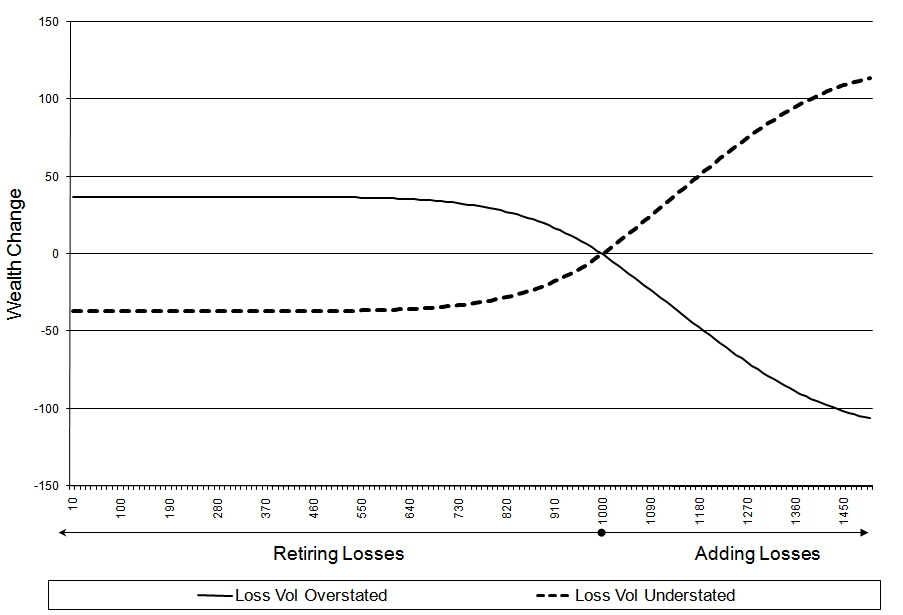
\includegraphics[type=png,ext=.png,read=.png,width=4.8in]{volover}}
\end{center}
\end{figure}

\begin{figure}\caption{Expected Loss and Volatility Deviations -- Same Direction\label{fig:bothsame}}
\begin{small}Examples of controlling shareholder wealth changes following capital structure swaps.  The solid line corresponds with the swaps illustrated in table \ref{tab:bothover} and the dashed line corresponds with the swaps illustrated in table \ref{tab:bothunder}.  Points on the left side of the graph correspond with swaps in which the firm issues equity and uses the proceeds to purchase reinsurance.  Points on the right side of the graph correspond with swaps in which the firm sells new policies and uses the proceeds to retire equity.\end{small}
\begin{center}
{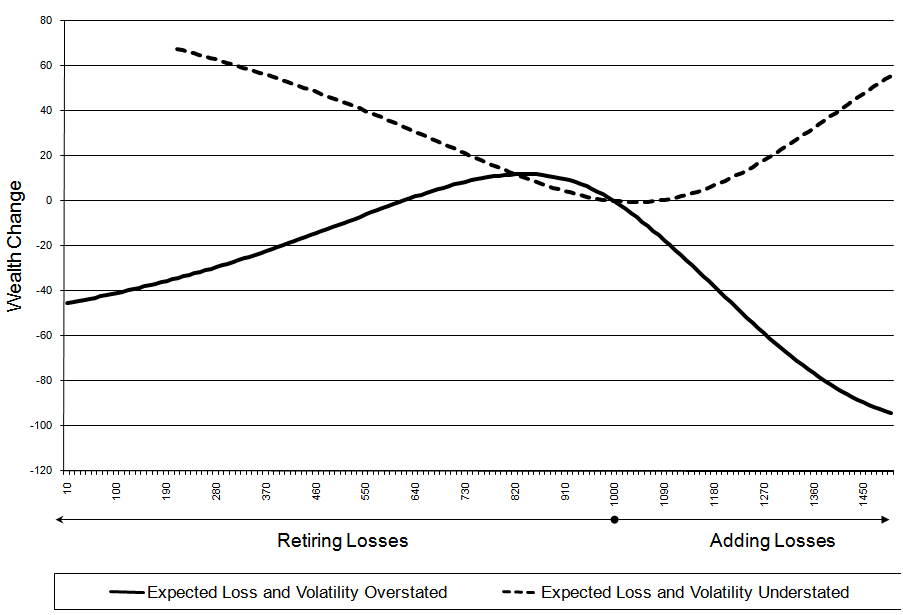
\includegraphics[type=png,ext=.png,read=.png,width=4.8in]{bothsame}}
\end{center}
\end{figure}

%\begin{figure}\caption{Expected Loss and Volatility Deviations -- Opposite Direction\label{fig:bothopp}}
%\begin{small}Examples of controlling shareholder wealth changes following capital structure swaps.  The solid line corresponds with the swaps illustrated in table \ref{tab:lossovervolunder} and the dashed line corresponds with the swaps illustrated in table \ref{tab:lossundervolover}.  Points on the left side of the graph correspond with swaps in which the firm issues equity and uses the proceeds to purchase reinsurance.  Points on the right side of the graph correspond with swaps in which the firm sells new policies and uses the proceeds to retire equity.\end{small}
%{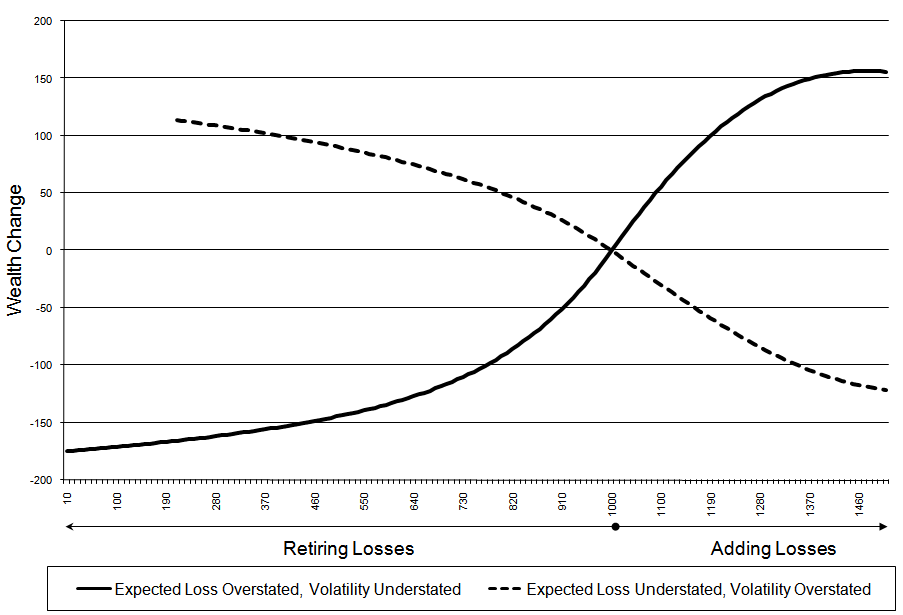
\includegraphics[type=png,ext=.png,read=.png,width=4.8in]{bothopp}}
%\end{figure}

\begin{figure}\caption{Asset/Loss Correlation Deviations\label{fig:corr}}
\begin{small}Examples of controlling shareholder wealth changes following capital structure swaps.  The solid line corresponds with the swaps illustrated in table \ref{tab:corrover} and the dashed line corresponds with the swaps illustrated in table \ref{tab:corrunder}.  Points on the left side of the graph correspond with swaps in which the firm issues equity and uses the proceeds to purchase reinsurance.  Points on the right side of the graph correspond with swaps in which the firm sells new policies and uses the proceeds to retire equity.\end{small}
\begin{center}
{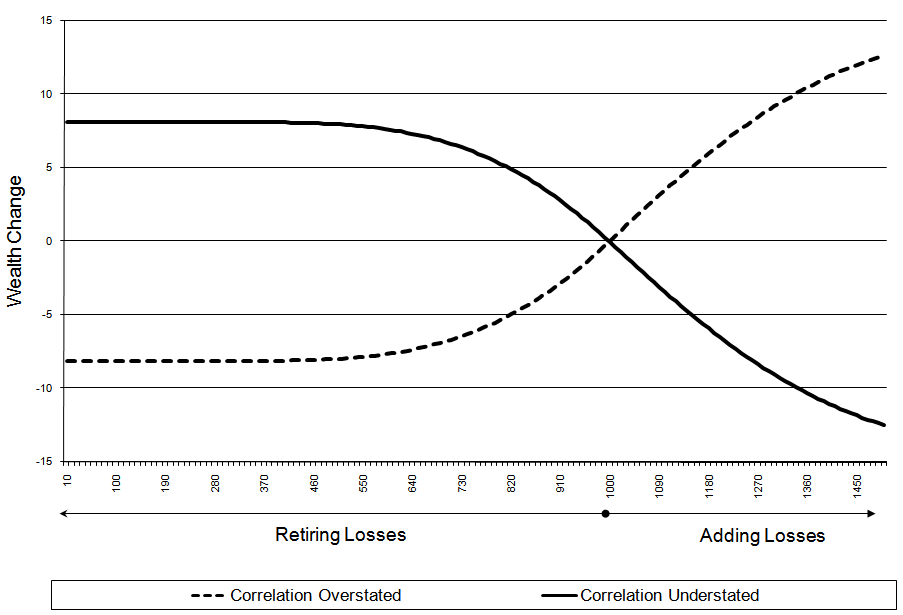
\includegraphics[type=png,ext=.png,read=.png,width=4.8in]{corr}}
\end{center}
\end{figure}

\section{Conclusion}\label{sec:conclusion}

Prior research has demonstrated that in most cases, firms that issue equity do so at the expense of the controlling shareholders.  Some research, however, has demonstrated that insurance company investors, in particular, may benefit from a different regulatory system that addresses many of the information asymmetry problems associated with new equity issues.  Further research has shown that insurers gain many advantages from purchasing reinsurance, including comparative advantages in risk-bearing and provision of real services.  When the managers can exploit risk aversion of potential policyholders to sell insurance at a premium to expected loss, they can increase the firm's leverage and use the proceeds to retire equity or invest in new projects.  At the same time, if managers can purchase value-adding reinsurance, they may choose to issue equity to raise the necessary cash to do so.

In this paper, we show that insurance companies have unique opportunities to engage in capital structure arbitrage by executing transactions that take advantage of market conditions and frictions. We use a Merton-Margrabe option pricing model to analyze the impact of an exchange of risky assets.  Contrary to the conventional rule, we show that controlling shareholders' wealth can increase when management engages in some swaps, issuing undervalued equity or selling cheap insurance policies. Finally, we show that an interior solution exists in some cases to maximize long-term shareholder value when both equity and loss liabilities are valued differently by noise traders and potential policyholders. 

These findings provide new rationale for the findings of \citet{akhigbe1997a}.  In addition to reduced information asymmetry due to regulation, differences in risk aversion, cost of real services and correlation between asset and loss portfolios can generate unique opportunities for capital structure swaps that are available to firms outside of the insurance and financial services sector.


\bibliographystyle{econometrica}
\bibliography{hilliard}
\end{document}



